%%%%%%%%%%%%%%%%%%%%%%%%%%%%%%%%%%%%%%%
% Wenneker Resume/CV
% LaTeX Template
% Version 1.1 (19/6/2016)
%
% This template has been downloaded from:
% http://www.LaTeXTemplates.com
%
% Original author:
% Frits Wenneker (http://www.howtotex.com) with extensive modifications by 
% Vel (vel@LaTeXTemplates.com)
%
% License:
% CC BY-NC-SA 3.0 (http://creativecommons.org/licenses/by-nc-sa/3.0/
%
%%%%%%%%%%%%%%%%%%%%%%%%%%%%%%%%%%%%%%

%----------------------------------------------------------------------------------------
%	PACKAGES AND OTHER DOCUMENT CONFIGURATIONS
%----------------------------------------------------------------------------------------

\documentclass[a4paper,12pt]{memoir} % Font and paper size

%%%%%%%%%%%%%%%%%%%%%%%%%%%%%%%%%%%%%%%%%
% Wenneker Resume/CV
% Structure Specification File
% Version 1.1 (19/6/2016)
%
% This file has been downloaded from:
% http://www.LaTeXTemplates.com
%
% Original author:
% Frits Wenneker (http://www.howtotex.com) with extensive modifications by 
% Vel (vel@latextemplates.com)
%
% License:
% CC BY-NC-SA 3.0 (http://creativecommons.org/licenses/by-nc-sa/3.0/)
%
%%%%%%%%%%%%%%%%%%%%%%%%%%%%%%%%%%%%%%%%%

%----------------------------------------------------------------------------------------
%	PACKAGES AND OTHER DOCUMENT CONFIGURATIONS
%----------------------------------------------------------------------------------------

\usepackage{XCharter} % Use the Bitstream Charter font
\usepackage[utf8]{inputenc} % Required for inputting international characters
\usepackage[T1]{fontenc} % Output font encoding for international characters

\usepackage[top=1cm,left=1cm,right=1cm,bottom=1cm]{geometry} % Modify margins

\usepackage{graphicx} % Required for figures

\usepackage{flowfram} % Required for the multi-column layout

\usepackage{url} % URLs

\usepackage[usenames,dvipsnames]{xcolor} % Required for custom colours

\usepackage{tikz} % Required for the horizontal rule

\usepackage{enumitem} % Required for modifying lists
\setlist{noitemsep,nolistsep} % Remove spacing within and around lists

\setlength{\columnsep}{\baselineskip} % Set the spacing between columns

% Define the left frame (sidebar)
\newflowframe{0.2\textwidth}{\textheight}{0pt}{0pt}[left]
\newlength{\LeftMainSep}
\setlength{\LeftMainSep}{0.2\textwidth}
\addtolength{\LeftMainSep}{1\columnsep}
 
% Small static frame for the vertical line
\newstaticframe{1.5pt}{\textheight}{\LeftMainSep}{0pt}
 
% Content of the static frame with the vertical line
\begin{staticcontents}{1}
\hfill
\tikz{\draw[loosely dotted,color=RoyalBlue,line width=1.5pt,yshift=0](0,0) -- (0,\textheight);}
\hfill\mbox{}
\end{staticcontents}
 
% Define the right frame (main body)
\addtolength{\LeftMainSep}{1.5pt}
\addtolength{\LeftMainSep}{1\columnsep}
\newflowframe{0.7\textwidth}{\textheight}{\LeftMainSep}{0pt}[main01]

\pagestyle{empty} % Disable all page numbering

\setlength{\parindent}{0pt} % Stop paragraph indentation

%----------------------------------------------------------------------------------------
%	NEW COMMANDS
%----------------------------------------------------------------------------------------

\newcommand{\userinformation}[1]{\renewcommand{\userinformation}{#1}} % Define a new command for the CV user's information that goes into the left column

\newcommand{\cvheading}[1]{{\Huge\bfseries\color{RoyalBlue} #1} \par\vspace{.6\baselineskip}} % New command for the CV heading
\newcommand{\cvsubheading}[1]{{\Large\bfseries #1} \bigbreak} % New command for the CV subheading

\newcommand{\Sep}{\vspace{1em}} % New command for the spacing between headings
\newcommand{\SmallSep}{\vspace{0.5em}} % New command for the spacing within headings

\newcommand{\aboutme}[2]{ % New command for the about me section
\textbf{\color{RoyalBlue} #1}~~#2\par\Sep
}
	
\newcommand{\CVSection}[1]{ % New command for the headings within sections
{\Large\textbf{#1}}\par
\SmallSep % Used for spacing
}

\newcommand{\CVItem}[2]{ % New command for the item descriptions
\textbf{\color{RoyalBlue} #1}\par
#2
\SmallSep % Used for spacing
}

\newcommand{\bluebullet}{\textcolor{RoyalBlue}{$\circ$}~~} % New command for the blue bullets
 % Include the file specifying document layout and packages

%----------------------------------------------------------------------------------------
%	NAME AND CONTACT INFORMATION 
%----------------------------------------------------------------------------------------

\userinformation{ % Set the content that goes into the sidebar of each page
\begin{flushright}
% Comment out this figure block if you don't want a photo
% \includegraphics[width=0.6\columnwidth]{photo.png}\\[\baselineskip] % Your photo
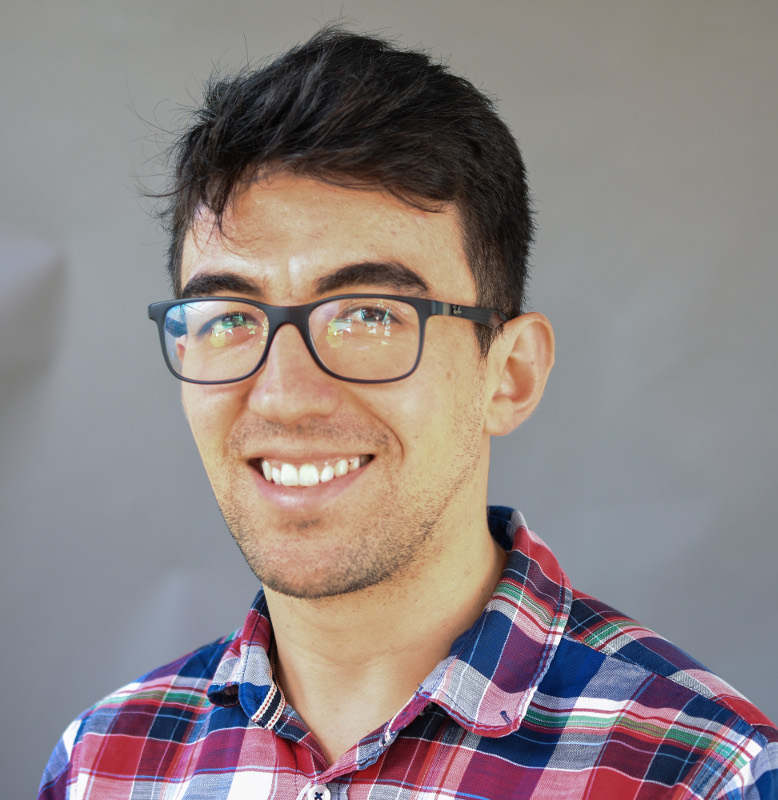
\includegraphics[width=0.7\columnwidth]{PhotoLinkedinshort.jpg}
\small % Smaller font size
Nikolay Prieto \\ % Your name
\scriptsize{\url{enprietop@unal.edu.co}} \\ % Your email address
% \url{www.johnsmith.com} \\ % Your URL
+57 (300) 350 1177 \\ % Your phone number
\Sep % Some whitespace
\textbf{Address} \\
Calle 12 # 3-05 \\ % Address 1
La Calera, Cundinamarca \\ % Address 2
Colombia \\ % Address 3
\vfill % Whitespace under this block to push it up under the photo
\end{flushright}
}

%----------------------------------------------------------------------------------------

\begin{document}

\userinformation % Print your information in the left column

\framebreak % End of the first column

%----------------------------------------------------------------------------------------
%	HEADING
%----------------------------------------------------------------------------------------

\cvheading{Nikolay Prieto} % Large heading - your name

\cvsubheading{Mechatronics Engineer} % Subheading - your occupation/specialization

%----------------------------------------------------------------------------------------
%	ABOUT ME
%----------------------------------------------------------------------------------------

\aboutme{About Me}{Ph.D. candidate with strong knowledge in product design, focused on human bio-mechanics especially, I have got work experience in project management and as a lecturer at the National University of Colombia. I have excellent skills in programming and physical computer modeling, good skills in personal relationships, leadership, responding flexibly and positively to changing situations, continuous learning autonomy, persistent and oriented to objectives. Nowadays, while I am finishing my Ph.D., I am looking for a job in the industry, research or academy.}

%----------------------------------------------------------------------------------------
%	EDUCATION
%----------------------------------------------------------------------------------------

\CVSection{Education}

%------------------------------------------------

\CVItem{2014 - current, Universidad Nacional de Colombia}{\textbf{Doctorate in Engineering.} \\
\textbf{Thesis title:} \textit{Passive Dynamic System for Energy Returning on Transtibial Prosthesis.} \\
\textbf{Grade Point Average:} 4.4/5.0 \\
\textbf{Modules Included:}
\begin{itemize}
    \item Biomechanical Engineering.
    \item Advanced Process of Manufacturing.
    \item Advanced Applications on Finite Element Analysis.
    \item Data Visualization and Machine Learning.
    \item Topology Optimization.
    \item Bio-inspired Optimization.
\end{itemize}}
%------------------------------------------------
\CVItem{2011 - 2014, Military University of Colombia}{M.Eng. in Mechatronics} \\
\textbf{Thesis title:} \textit{Design, simulation and manufacturing of a high impact prosthesis for lower limb Colombian amputees.} \\
\textbf{Grade Point Average:} 4.5/5.0 \\
\textbf{Modules Included:}
\begin{itemize}
    \item Advanced Strategies in Control Engineering.
    \item Non-linear System Analysis.
    \item Embedded Systems.
    \item Materials and Manufacturing.
    \item Finite Element Analysis.
\end{itemize}

\CVItem{2004 - 2009, San Buenaventura University, Colombia}{BS. in Mechatronics Engineering.}
%------------------------------------------------

\Sep % Extra whitespace after the end of a major section

%----------------------------------------------------------------------------------------
%	EXPERIENCE
%----------------------------------------------------------------------------------------

\CVSection{Experience}

%------------------------------------------------

\CVItem{June 2018 - present, \textit{Research Assistant}, Indiana University Purdue University-Indianapolis (IUPUI)}{
Detailed achievements:
\begin{itemize}
    \item Design of biomedical devices.
    \item Perform topology optimization algorithms.
    \item Additive manufacturing.
    \item CAD design.
    \item Non-linear FEA simulations.
    \item Injection molding.
\end{itemize}
}

%------------------------------------------------
% ----------------------------
%	NEW PAGE DELIMITER
%	Place this block wherever you would like the content of your CV to go onto the next page
%----------------------------------------------------------------------------------------

\clearpage % Start a new page

\userinformation % Print your information in the left column

\framebreak % End of the first column
%------------------------------------------------------------

\CVItem{Feb. 2015 - June 2018, \textit{Lecturer}, Universidad Nacional de Colombia}{\textbf{Subject given}: Interdisciplinary projects workshop. \\
Mentoring and counseling in projects development for students of
different careers in the school of engineering.}



\CVItem{Feb. 2009 - Sep. 2014, \textit{Research and Development projects coordinator}, Military Industry of Colombia (INDUMIL)}{Administrative and technical management of projects focused on research and technological development in the defense field.
The duties involved were: Management, monitoring, researching, technological assessment, industrial property, engineering design and prototypes manufacturing, among other activities of projects related to mobile TV operated robotics, prosthetics for lower and upper limbs, command and control systems, military vehicles, etc.}
%----------------------------------------------------------------------------------------
%	COMMUNICATION SKILLS
%----------------------------------------------------------------------------------------

\CVSection{Communication Skills}

%------------------------------------------------

\CVItem{2013, \textit{Oral Presentation}, ESSS-CAE Industry Aerospace and
Defense congress}{\textbf{Talk title:} Determination of internal pressure, velocity and recoil in water
jet cannons with AutoDYN.}

%------------------------------------------------

\Sep % Extra whitespace after the end of a major section

%----------------------------------------------------------------------------------------
%	SKILLS
%----------------------------------------------------------------------------------------

\CVSection{Software Development Skills}

%------------------------------------------------

\CVItem{Programming}
{\begin{tabular}{p{0.2\textwidth} p{0.2\textwidth} p{0.2\textwidth}}
\bluebullet Python &  \bluebullet Matlab & \bluebullet Shell\\
\end{tabular}}

%------------------------------------------------

\CVItem{Computer Software}
{\begin{tabular}{p{0.2\textwidth} p{0.2\textwidth} p{0.2\textwidth}}
 \bluebullet Windows &  \bluebullet Linux & \bluebullet LS-DYNA\\
 \bluebullet ANSYS &  \bluebullet Inventor & \bluebullet AutoCAD\\
 \bluebullet ALTIUM Designer & \\
\end{tabular}}

%-----------------------------------

\CVItem{Open Source}

{\begin{tabular}{p{0.2\textwidth} p{0.2\textwidth} p{0.2\textwidth}}
\bluebullet \LaTeX &  \bluebullet Opensim & \bluebullet Octave\\
\bluebullet FeBio &  \bluebullet Gmsh & \bluebullet G-code\\
\end{tabular}}
%------------------------------------------------

\Sep % Extra whitespace after the end of a major section
%----------------------------------------------------------------------------------------
%	AWARDS
%----------------------------------------------------------------------------------------

\CVSection{Awards}

%------------------------------------------------

\CVItem{2015, \textit{Postgraduate Scholarship}, Universidad Nacional de Colombia}{Best GPA in the PhD programme.}

\CVItem{2014, \textit{Postgraduate Scholarship}, COLCIENCIAS}{Grantee for all the PhD academic programme.}

\CVItem{2011, \textit{Postgraduate Scholarship}, Military Industry of Colombia}{ Masters Scholarship.}
%------------------------------------------------

\Sep % Extra whitespace after the end of a major section
%----------------------------------------------------------------------------------------
%	LANGUAGES
%----------------------------------------------------------------------------------------
\CVSection{Languages.}
\begin{itemize}
    \item Spanish (Mother Tongue)
    \item English (B2 level TOEFL certified)
\end{itemize}

\Sep

%----------------------------------------------------------------------------------------
%	INTERESTS
%----------------------------------------------------------------------------------------

\CVSection{Interests}

%------------------------------------------------

\CVItem{Professional}{Education, Research, Programming, Biomechanics, FEA, Computer Science, 3D printing.}

%------------------------------------------------

\CVItem{Personal}{Volleyball, cooking, travelling, running.}

%------------------------------------------------

\Sep % Extra whitespace after the end of a major section

%----------------------------------------------------------------------------------------

\end{document}
